

\documentclass{article}[14pt, oneside, a4paper, times]

\usepackage[utf8]{inputenc}
\usepackage[english]{babel}
\usepackage[T1]{fontenc}
\usepackage{epsfig}           % para incluir figuras
\usepackage{subfig}
\usepackage{graphicx}
\usepackage{setspace}
\usepackage{vmargin}
\usepackage{algorithm}
\usepackage{algorithmic}
\usepackage{amsfonts} 
\usepackage{amssymb}


\setpapersize [portrait]{A4}
\setmarginsrb {30mm} % margem esquerda
              {10mm} % margem topo
             {30mm} % margem direita
            {20mm} % margem pé
           {2ex}  % altura do espaco para cabeçalho
           {5ex}  % espaço entre fim do cabeçalho e início do texto
          {0pt}  % altura do espaço para rodapé
         {20mm}  % espaço entre fim do texto e fim do rodapé

\doublespacing

%=======================================================================
\pagestyle{myheadings}
\begin {document}

\title{Pre-Processing and Feature Extraction 
\\ \large Global Features}
\author{Luiz S. Oliveira and Marisa Morita  
\\
\vspace {-10pt}
Federal University of Parana (UFPR)\\
\vspace {-10pt}
Department of Informatics (DInf)\\
\vspace {-10pt}
R. Rua Cel. Francisco H. dos Santos, 100, Curitiba, PR, Brazil \\
lesoliveira@inf.ufpr.br \\ 
}


\date{}
\maketitle
%\vspace{-2\baselineskip}
\thispagestyle{empty}

%\begin{abstract}

%bla bla


%\end{abstract}

%%%%%%%%%%%%%%%%%%%%%%%%%%%%%%%%%%%%%%%%%%%%%%%%%%%%%%%%%%%%%%%%%%%%%%%%%%%%%%%%%
% Introduction 
%%%%%%%%%%%%%%%%%%%%%%%%%%%%%%%%%%%%%%%%%%%%%%%%%%%%%%%%%%%%%%%%%%%%%%%%%%%%%%%%%
\section{Introduction} 

This report describes the activities performed in the last month, which were devoted to the implementation of the global features for month recognition. Besides feature extraction, some routines of pre-processing and segmentation were also implemented. These routines, which have been proved efficient for word recognition, will be used for other feature sets we plan to develop latter in the project. 

The source code is available in the SVN repository. Before compiling the code make sure to update the \textsf{PPROJ} variable in the \textsf{Make\_orand\_globfeat} file available in the directory \textsf{./tools/orand/batch/feature/gen} and also to update the defines in the \textsf{global.h} file, available in the directory \textsf{./tools/orand/inter/include}. To compile the source code use

\begin{verbatim}
make -f Make_orand_globfeat
\end{verbatim}

\noindent And to execute the program, type

\begin{verbatim}
./orand_globfeat feat1 globf
\end{verbatim}

The program generates three different files for training, validation and testing, respectively. Those files are located in the directory \textsf{./tools/orand/param/train/feat1} and \textsf{./tools/orand/param/test/feat1}.


In the next sections we describe the main modules implemented to detect and extract the feature vector based on global primitives. 

\section{Pre-Processing}

As we will see later in this report, the feature extraction technique is based on a segmentation algorithm that detects some key points in the upper and lower contour. These points serve as anchor for the feature extraction process. It has been demonstrated \cite{Morita2004} that the segmentation algorithm works better for slant free words. For this reason we have implemented a simple, but efficient, slant correction technique. It corrects the slant using a shear transformation defined in the following Equation

\[
\left\{
\begin{array}{ll}
 x' =&  x - (y \times \tan(\theta))   \\
 y' =&  y    \\
   
\end{array}
\right.
\]

Another pre-processing that has been proved useful for character recognition is the smoothing. In our implementation we have used the technique proposed in \cite{Strathy93}, which passes a $3 \times 3$ mask (Figure \ref{mask:fig}) over the image starting in the lower right corner and processes each row moving upwards row by row. The pixel in the center of the mask is the target. Pixels overlaid by squares marked ``X'' are ignored. If the pixels overlaid by the squares marked ``='' all have the same value, i.e., all zero, or all one, then the target pixel is forced to match them, otherwise it is not changed. This test is done four times for each target pixel, once for each possible rotation of the mask. The result is that single-pixel indentations in all edges are filled and single-pixel bumps are removed

\begin{figure}[htbp]
   \centering
   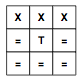
\epsfig{file=mask, width=2.5cm}
   \caption{3 $\times$ 3 mask used for smoothing.}
   \label{mask:fig}
\end{figure}

\section{Reference Lines}

Ascenders, descenders, and loops are good primitives to recognise handwritten words. The discriminative power can be boosted if the location information is added to the feature vector. To be able to do that, before detecting such primitives it is necessary to define some reference lines. In our case, we have defined five reference lines using simple density histograms: (1) median line, (2) upper baseline, (3) lower baseline, (4) upper line, and (5) lower line, which delimit the upper, median, and lower regions. Usually, the median region contains the lowercase letters and the upper and lower regions possess the ascenders and descenders. Figure \ref{reflines:fig} depicts those lines.

\begin{figure}[htbp]
   \centering
   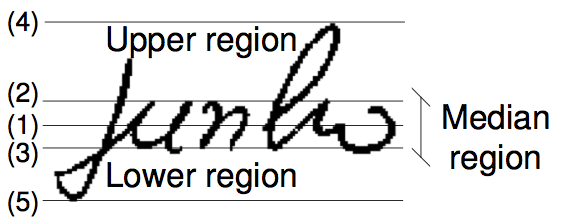
\epsfig{file=reflines, width=6cm}
   \caption{Five reference lines used for feature extraction \cite{Marisa03}}
   \label{reflines:fig}
\end{figure}

\section{Segmentation into Graphemes}

Segmenting a word into characters is a very complicated task, mainly due to the variability of the handwriting. With this in mind, for segmentation-based word recognition techniques it is important to design a segmentation algorithm that produces several segmentation points where the optimal ones are determined during recognition.

The algorithm we have used uses contour information, loops, reference lines and some heuristics to identify the segmentation points. As output, the algorithm provides a sequence of graphemes where each one may be a correctly segmented, under-segmented or an over-segmented character. Besides the segmentation points produced by the algorithm, a word may have some natural segmentation points. An example of the different segmentation points in presented in Figure \ref{segpoints:fig}.

\begin{figure}[htbp]
   \centering
   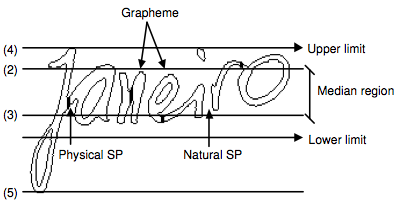
\epsfig{file=segpoints, width=8cm}
   \caption{Types of segmentation points that may generate graphemes \cite{Marisa03}}
   \label{segpoints:fig}
\end{figure}

\section{Feature Extraction}

Ascenders, descenders, and loops are detected through the upper contour maxima, lower contour minima, and secondary contours, respectively. These features are usually located in the upper and lower regions, respectively. Because of the variability of the handwriting, it is quite difficult to detect such regions, though. 

After detecting the aforementioned features, they are classified into big or small primitives according to their position (maxima and minima) in such regions. The region of small ascenders (descenders) is situated between the upper (lower) limit and this limit decreased (increased) by 40\% of the median region height. The remaining of the upper (lower) region is considered the area of big ascenders (descenders). In both cases, the threshold we have used was chosen based on experimentation carried out on the validation set. Therefore, if an upper contour maximum (lower contour minima) is located in the small or big region, it corresponds to a small or big ascender (descender) respectively.

Loops can be identified in any of the three regions (upper, median, and lower) depending on the position of their gravity centres. Loops belonging to the median region are encoded in two ways (big or small). The big loops are those ones greater than the half of the median region height. Thus, the combination of the foregoing primitives plus a primitive that determines if a grapheme does not contain ascender, descender, and loop produces a 20-symbol alphabet. Table \ref{symbols:tab} describes the symbols that compose the global feature vector.


\begin{table} [ht!]
\caption {Description of the 20-symbol alphabet}
\begin{center}
\begin{tabular}{ll} \hline 
 \multicolumn{1}{c}{Symbol}&
 \multicolumn{1}{c}{Description} \\ \hline

O & Big loop in the median region \\
o & Small loop in the median region \\
H & Big ascender \\
h & Small ascender \\
B & Big descender\\
b & Small descender \\
L & Big ascender and a loop in the upper region\\
l & Small ascender and a loop in the upper region\\
Z & Big or small descender and a loop in the superior region\\
- & Absence of ascender, descender, and loops\\
D & Big ascender and a big or small loop in the median region\\
d & Small ascender and a big loop in the median region\\
s & Small ascender and a small loop in the median region\\
Q & Big descender and a big or small loop in the median region\\
q & Small descender and a big or small loop in the median region\\
K & Big or small ascender, a loop in the upper region, \\
  & and a big or small loop in the median region\\
G & Big or small descender, a loop in the upper region, \\
  & and a big or small loop in the median region\\
M & Big or small ascender and descender\\
F & Big or small descender and a loop in the upper or lower region\\
x & Big or small descender and a big or small loop in the median region\\ \hline


\end{tabular}
\label{symbols:tab}
\end{center}
\end{table}

Figure \ref{agosto:fig} shows an image with its respective global feature vector. 

\begin{figure}[htbp]
   \centering
   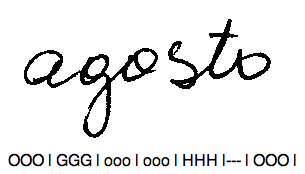
\epsfig{file=agosto, width=6cm}
   \caption{Month image with its respective global feature vector}
   \label{agosto:fig}
\end{figure}


\section{Conclusions}

In this report we have described the first feature set  developed to recognise handwritten words. It is a segmentation-based feature set that takes into account holistic features such as ascenders, descenders and loops. Our next activity consists in implementing and training a HMM-based classifier and train it using the described feature set.


\bibliographystyle{IEEEbib}
\bibliography{refer}



\end{document}



